\chapter{Analisi dei risultati} \label{1cap:analisi}
% [titolo ridotto se non ci dovesse stare] {titolo completo}
%



In questo capitolo saranno descritti i risultati ottenuti dall'implementenzione dei vari modelli di machine learning realizzati.
Una delle prime metriche prese in considerazione è l'accuratezza ottenuta dai vari modelli implementati, quest'ultima da come si evince dalla figura \ref{fig:Accuracy} ha registrato risultati molto alti per tutti i modelli implementati, nonostante ciò il classificatore che registrato una maggiore accuratezza è stato il Random forest con un risultato di \numprint{0.89}, mentre il risultato peggiore l'ha ottenuto il classificatore SVM con un risultato di \numprint{0.75}.

\begin{figure}[!htb]
    \centering
    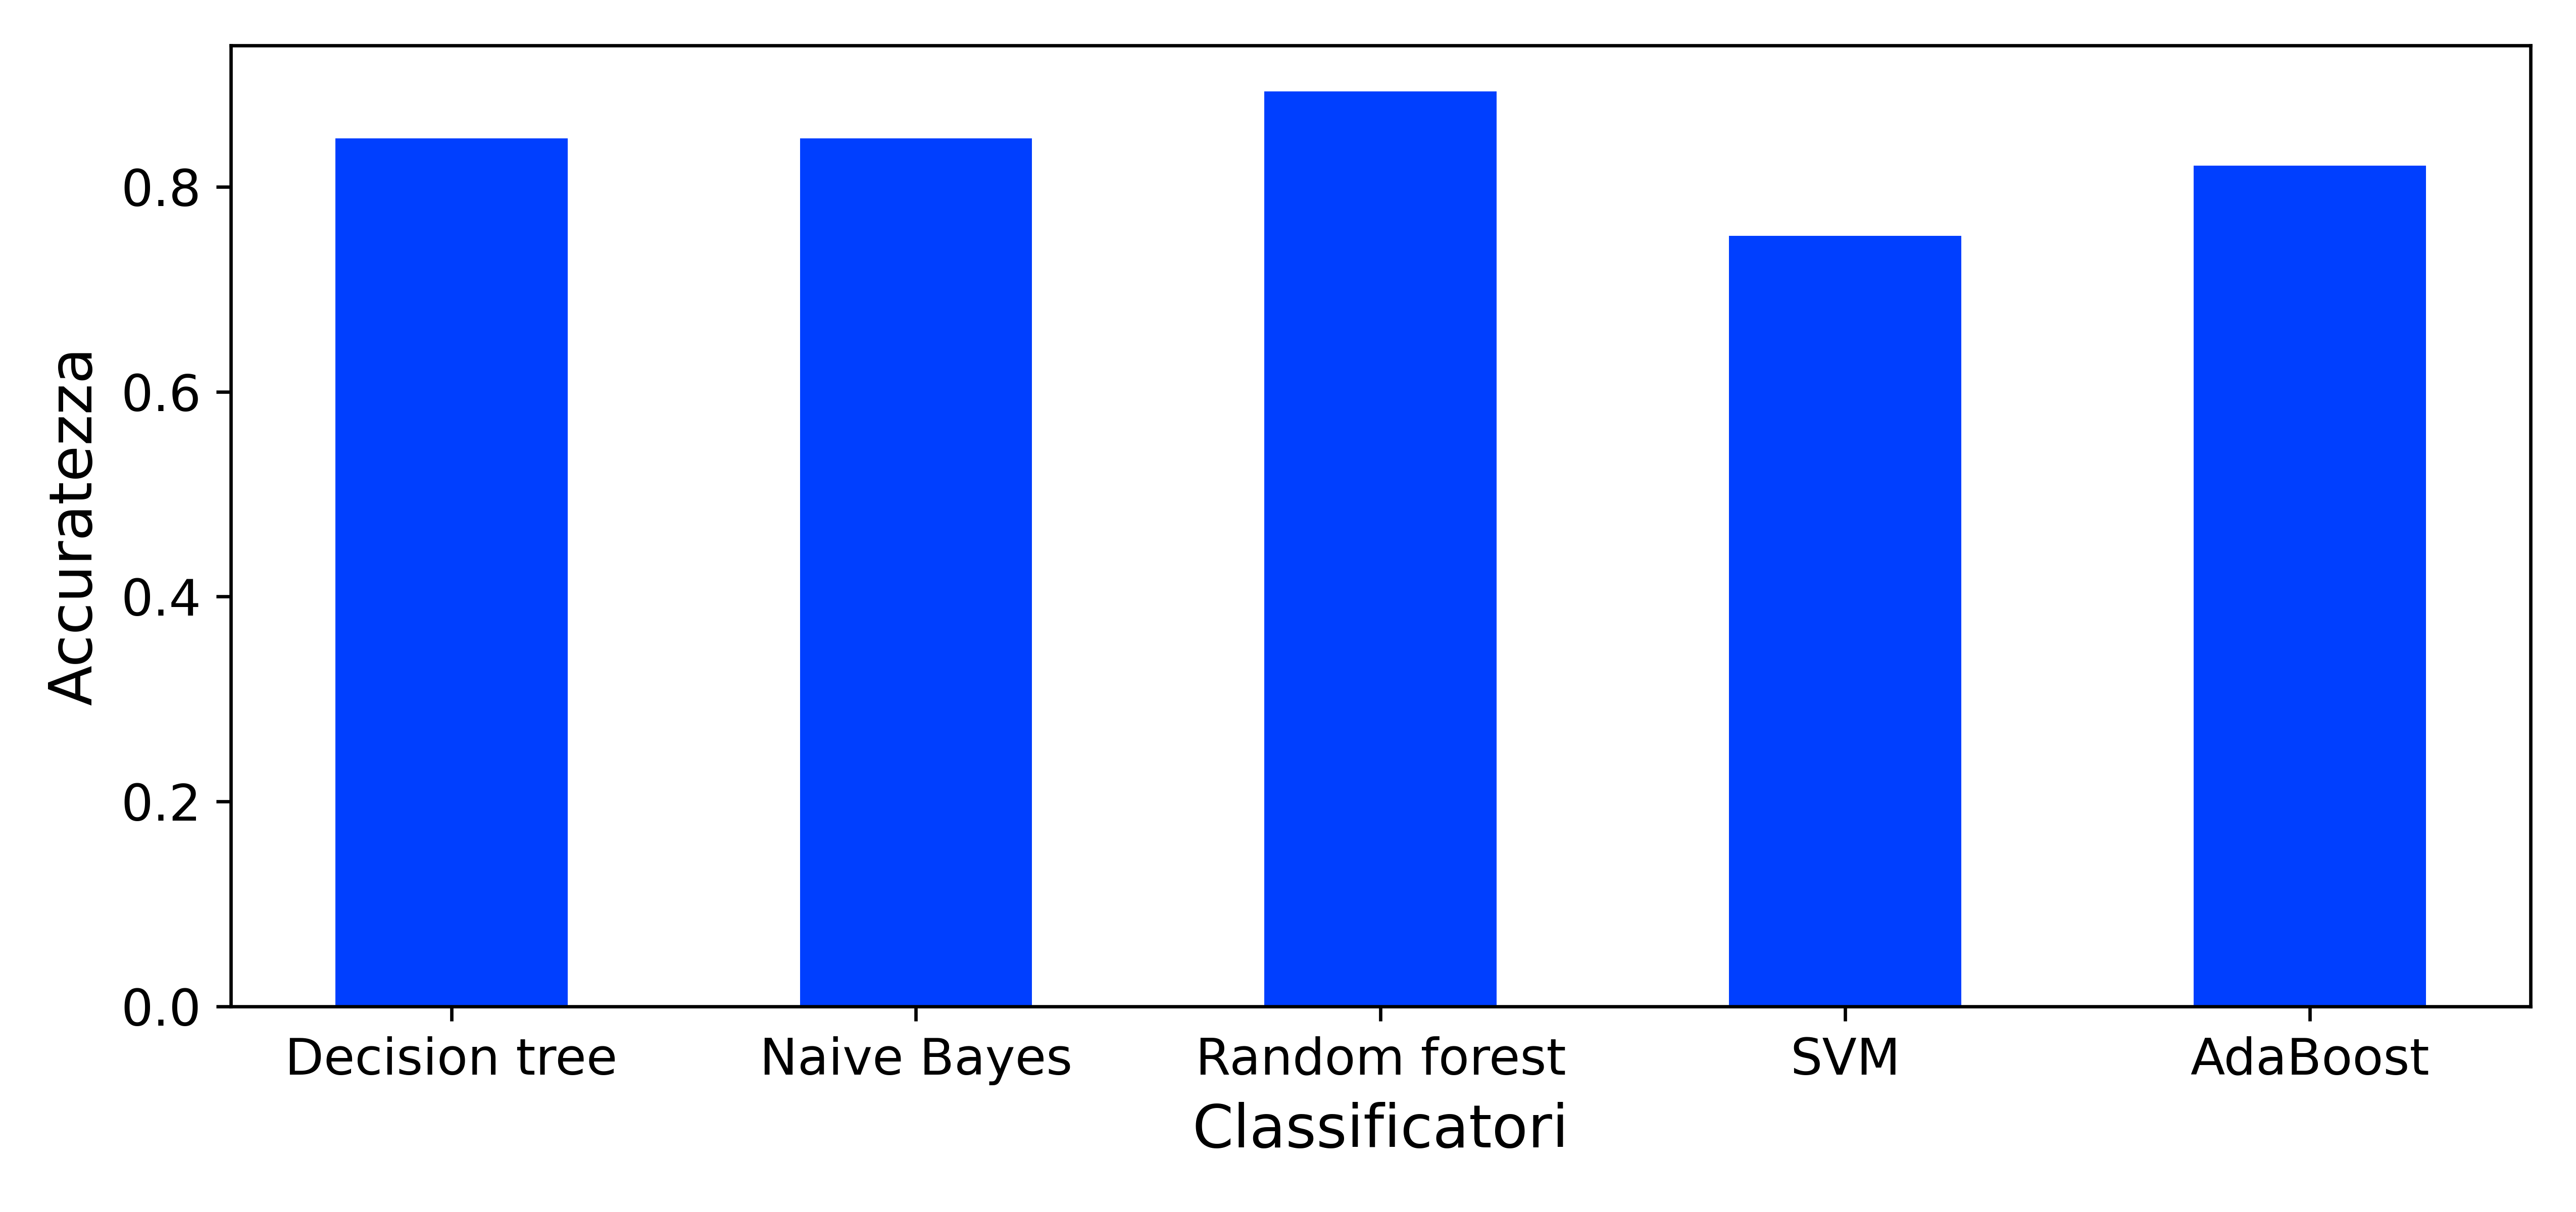
\includegraphics[scale=0.7]{../figure/Accuracy.png}
    \caption{Accuratezza classificatori}
    \label{fig:Accuracy}
\end{figure}

Successivamente ho preso in considerazione Precision e recall, quest'ultime mi danno la possibilità di analizzare più informazioni rispetto all'accuratezza, e inoltre mi permettono di avere una visione più completa delle prestazioni dei modelli implementati. Dalla tabella \ref{tab:PrecisionRecall} possiamo notare che in generale tutti i modelli hanno ottenuto risultati molto buoni per la predizione di file non vulnerabili, ma risultati poco precisi per la predizione di file vulnerabili, tra i diversi dati notiamo che il livello di precisione più alto raggiunto è stato di \numprint{0.34} per i file vulnerabili e \numprint{0.98} per i file non vulnerabili risultati ottenuti entrambi dal classificatore Random forest, mentre il livello di precisione più basso è stato ottenuto dal classificatore Naive Bayes con \numprint{0.08} per i file vulnerabili e \numprint{0.95} per i file non vulnerabili. \newline
\begin{table}[h]
    \centering
    \begin{tabular}{p{7cm}|r|r}
        \rowcolor{black}
        \textcolor{white}{\textbf{PREDIZIONE}} & \textcolor{white}{\textbf{PRECISION}} & \textcolor{white}{\textbf{RECALL}}\\  \multicolumn{3}{>{\columncolor{lightgray}}c}{\textbf{Decision tree}}\\
         File vulnerabili & \numprint{0.26} & \numprint{0.71}\\
         File non vulnerabili & \numprint{0.98} & \numprint{0.86}\\
         \multicolumn{3}{>{\columncolor{lightgray}}c}{\textbf{Naive Bayes}}\\
         File vulnerabili & \numprint{0.08} & \numprint{0.71}\\
         File non vulnerabili & \numprint{0.95} & \numprint{0.43}\\
         \multicolumn{3}{>{\columncolor{lightgray}}c}{\textbf{Random forest}}\\
         File vulnerabili & \numprint{0.34} & \numprint{0.71}\\
         File non vulnerabili & \numprint{0.98} & \numprint{0.91}\\
         \multicolumn{3}{>{\columncolor{lightgray}}c}{\textbf{SVM}}\\
         File vulnerabili & \numprint{0.14} & \numprint{0.53}\\
         File non vulnerabili & \numprint{0.96} & \numprint{0.77}\\
         \multicolumn{3}{>{\columncolor{lightgray}}c}{\textbf{AdaBoost}}\\
         File vulnerabili & \numprint{0.20} & \numprint{0.59}\\
         File non vulnerabili & \numprint{0.97} & \numprint{0.84} \\
    \end{tabular}
    \caption{Precision e Recall}
    \label{tab:PrecisionRecall}
\end{table}

Se guardiamo le prestazioni in termini di recall dei diversi modelli notiamo che il livello più alto per i file vulnerabili è di \numprint{0.71} ottenuto da tre classificatori diversi, mentre per i file non vulnerabili il risultato migliore è stato ottenuto dal Random forest con un livello di \numprint{0.91}, i risultati più bassi invece per i file vulnerabili sono stati registrati da SVM con \numprint{0.53}, mentre per i file non vulnerabili il livello più basso è stato di \numprint{0.43} ottenuto da Naive Bayes.
Attraverso la tabella \ref{tab:PrecisionRecall} è anche possibile notare le differenze in termini prestazionali dei vari classificatori, in particolare notiamo che in generale il classificatore con risultati più precisi è stato il Random forest seguito dal Decision tree, mentre il classificatore con risultati peggiori è stato il Naive Bayes, il quale ha registrato gli esiti più bassi per la predizione di file vulnerabili, registrando un grado di precisione molto basso. \newline
Dalla figura \ref{fig:F-measure} notiamo i risultati ottenuti in termini di F-measure dai diversi classificatori, questa misura attraverso un unico valore di permette di avere una visione più sintetica dei diversi risultati ottenuti dai classificatori, da questa misura notiamo che il classificatore che ha registrato maggiori prestazioni è stato il Random forest con un valore pari a \numprint{0.46}, mentre i risultati peggiori sono stati ottenuti dal classificatore SVM con \numprint{0.22}.

\begin{figure}[h]
    \centering
    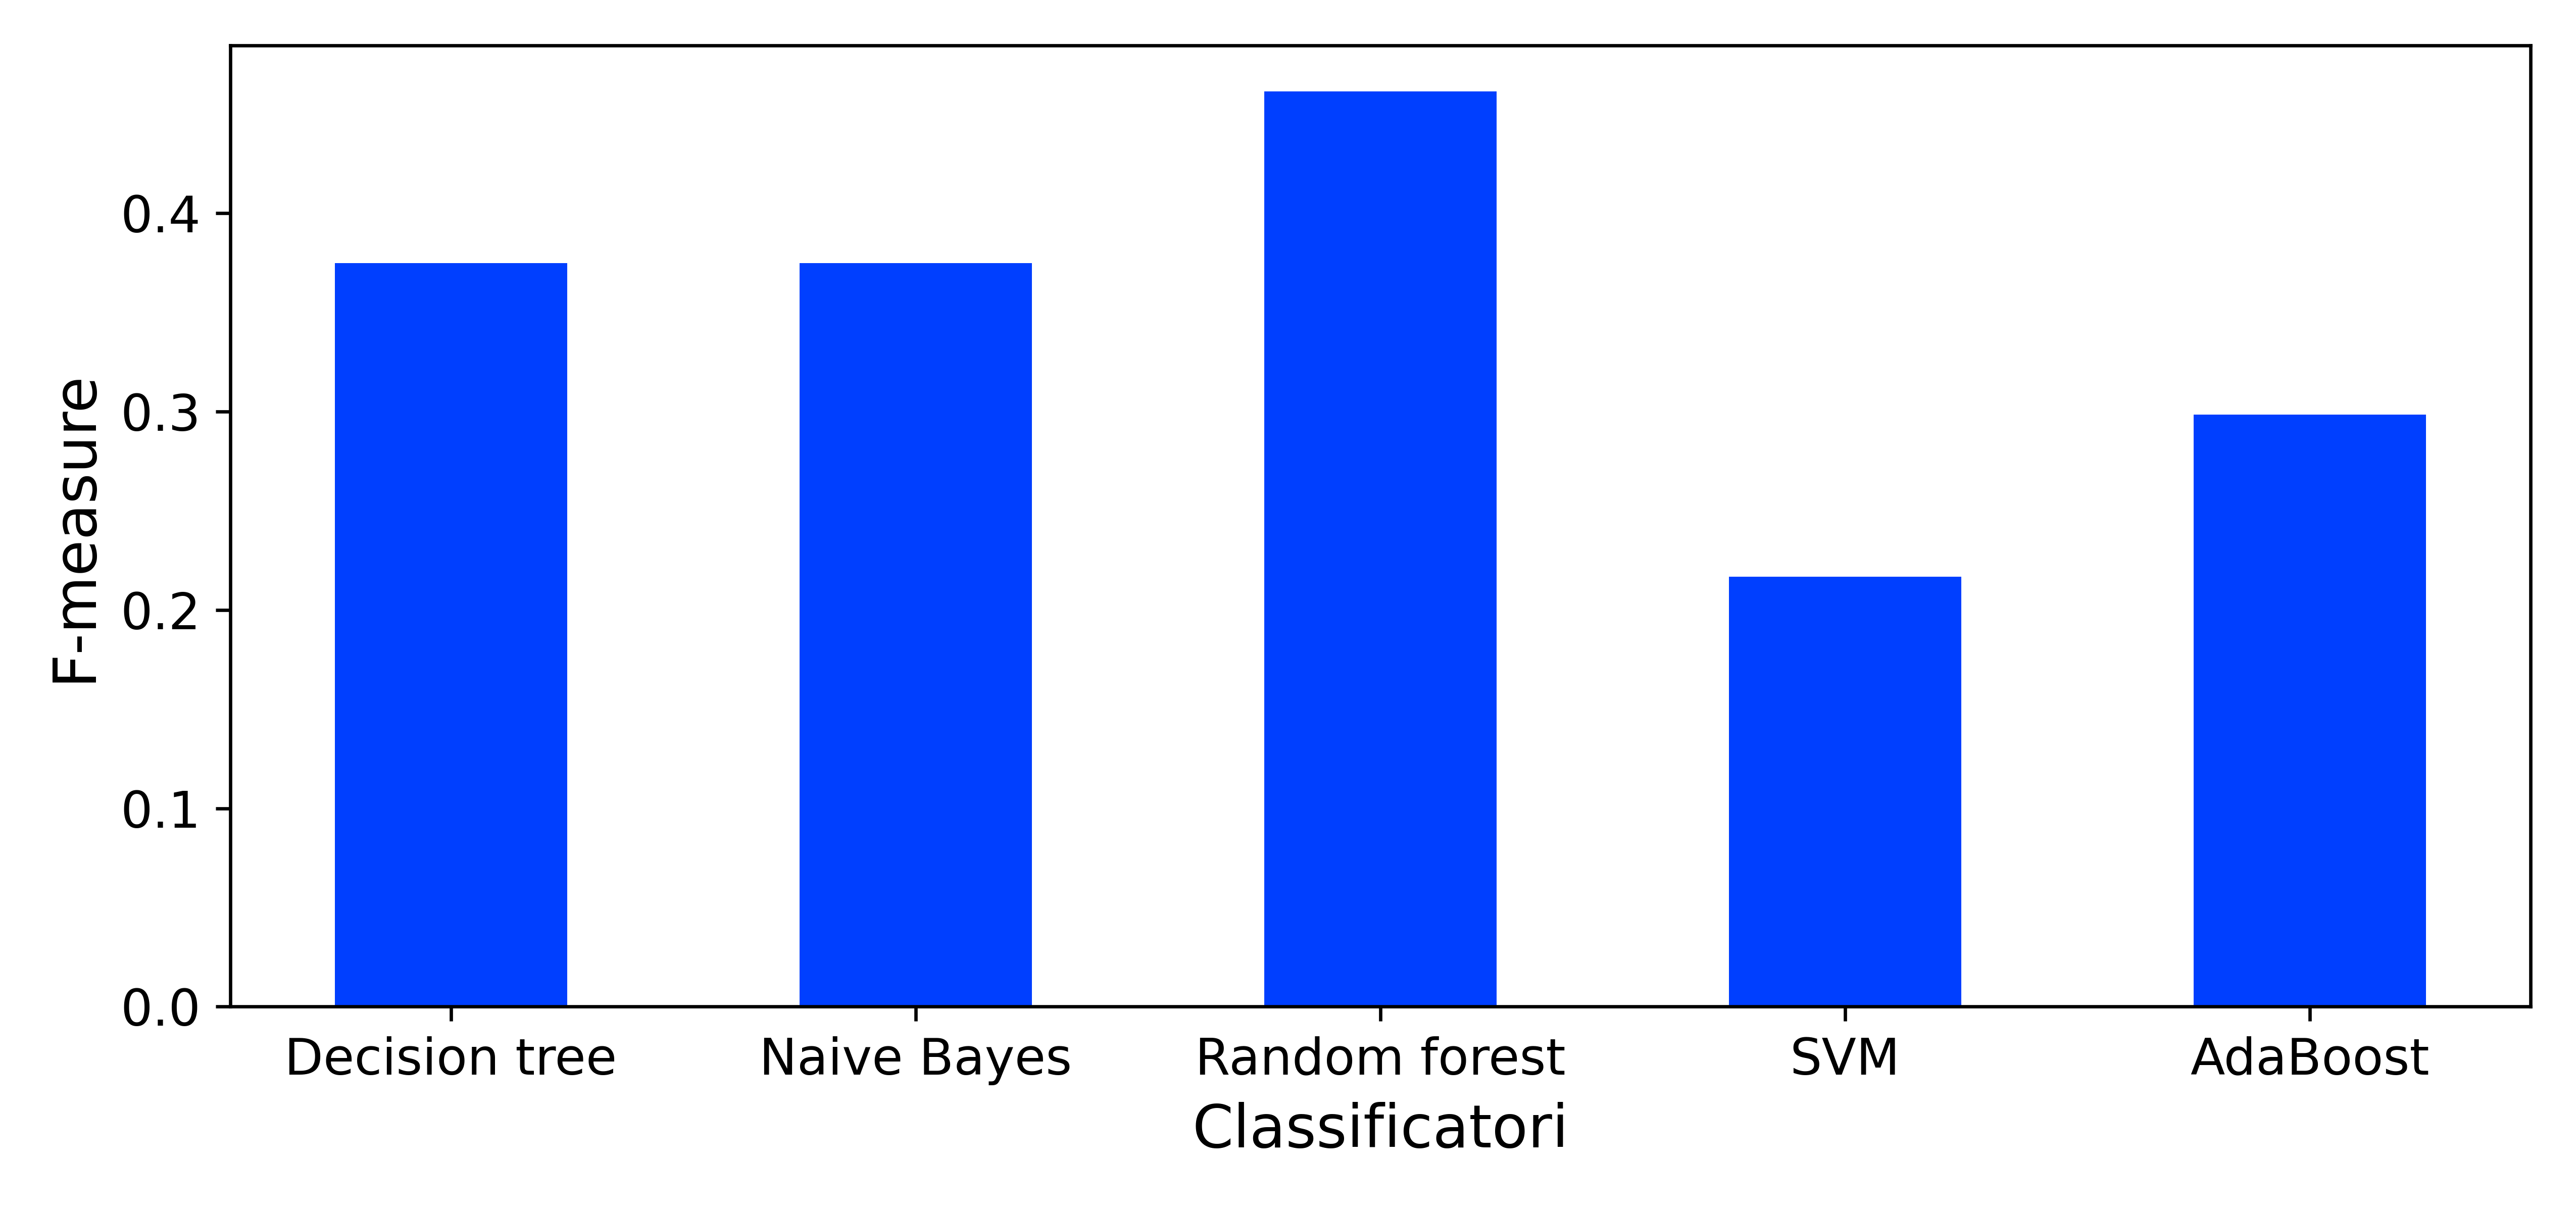
\includegraphics[scale=0.7]{../figure/F-measure.png}
    \caption{F-measure classificatori}
    \label{fig:F-measure}
\end{figure}


Confrontando le figure \ref{fig:Accuracy} e \ref{fig:F-measure} si possono notare risultati molto contrastanti tra F-measure e accuratezza, questa differenza è dovuta alla natura stessa del valore dell'accuratezza, quest'ultimo come descritto nel capitolo \ref{1cap:design} mette in relazione tutte le predizioni corrette con tutte le predizioni fatte dal modello in fase di validazione, è possibile comprendere questi esiti notando che il problema affrontato è fortemente sbilanciato ed i vari classificatori si comportano molto bene nella predizione dei file non vulnerabili, quindi durante la fase di validazione gran parte dei file presi in considerazione per la predizione sono file non vulnerabili, tutto ciò implica che il numero totale di predizioni esatte aumenta incrementando anche il livello di accuratezza.

Di particolare importanza durante la fase di validazione di un modello di predizione è visualizzare e analizzare la matrice di confusione ottenuta dalla validazione del modello, quest'ultima ha lo scopo di mettere in relazione tutte le predizioni che il modello ha eseguito con tutti i risultati reali del test selezionato per la validazione, nelle seguenti figure \ref{fig:CMNB}, \ref{fig:CMDT}, \ref{fig:CMRF}, \ref{fig:CMSVMe} e \ref{fig:CMAB}, sono stati riportati tutte le matrici di confusione di tutti i modelli implementati in questo studio. Leggendo questi dati possiamo notare che questi riflettono molto bene i dati analizzati precedentemente sopratutto valori di precision e recall analizzati nella tabella \ref{tab:PrecisionRecall}, inoltre ci permettono anche di comprendere il motivo di alcuni risultati ottenuti.
\begin{figure}[!ht]
\centering
    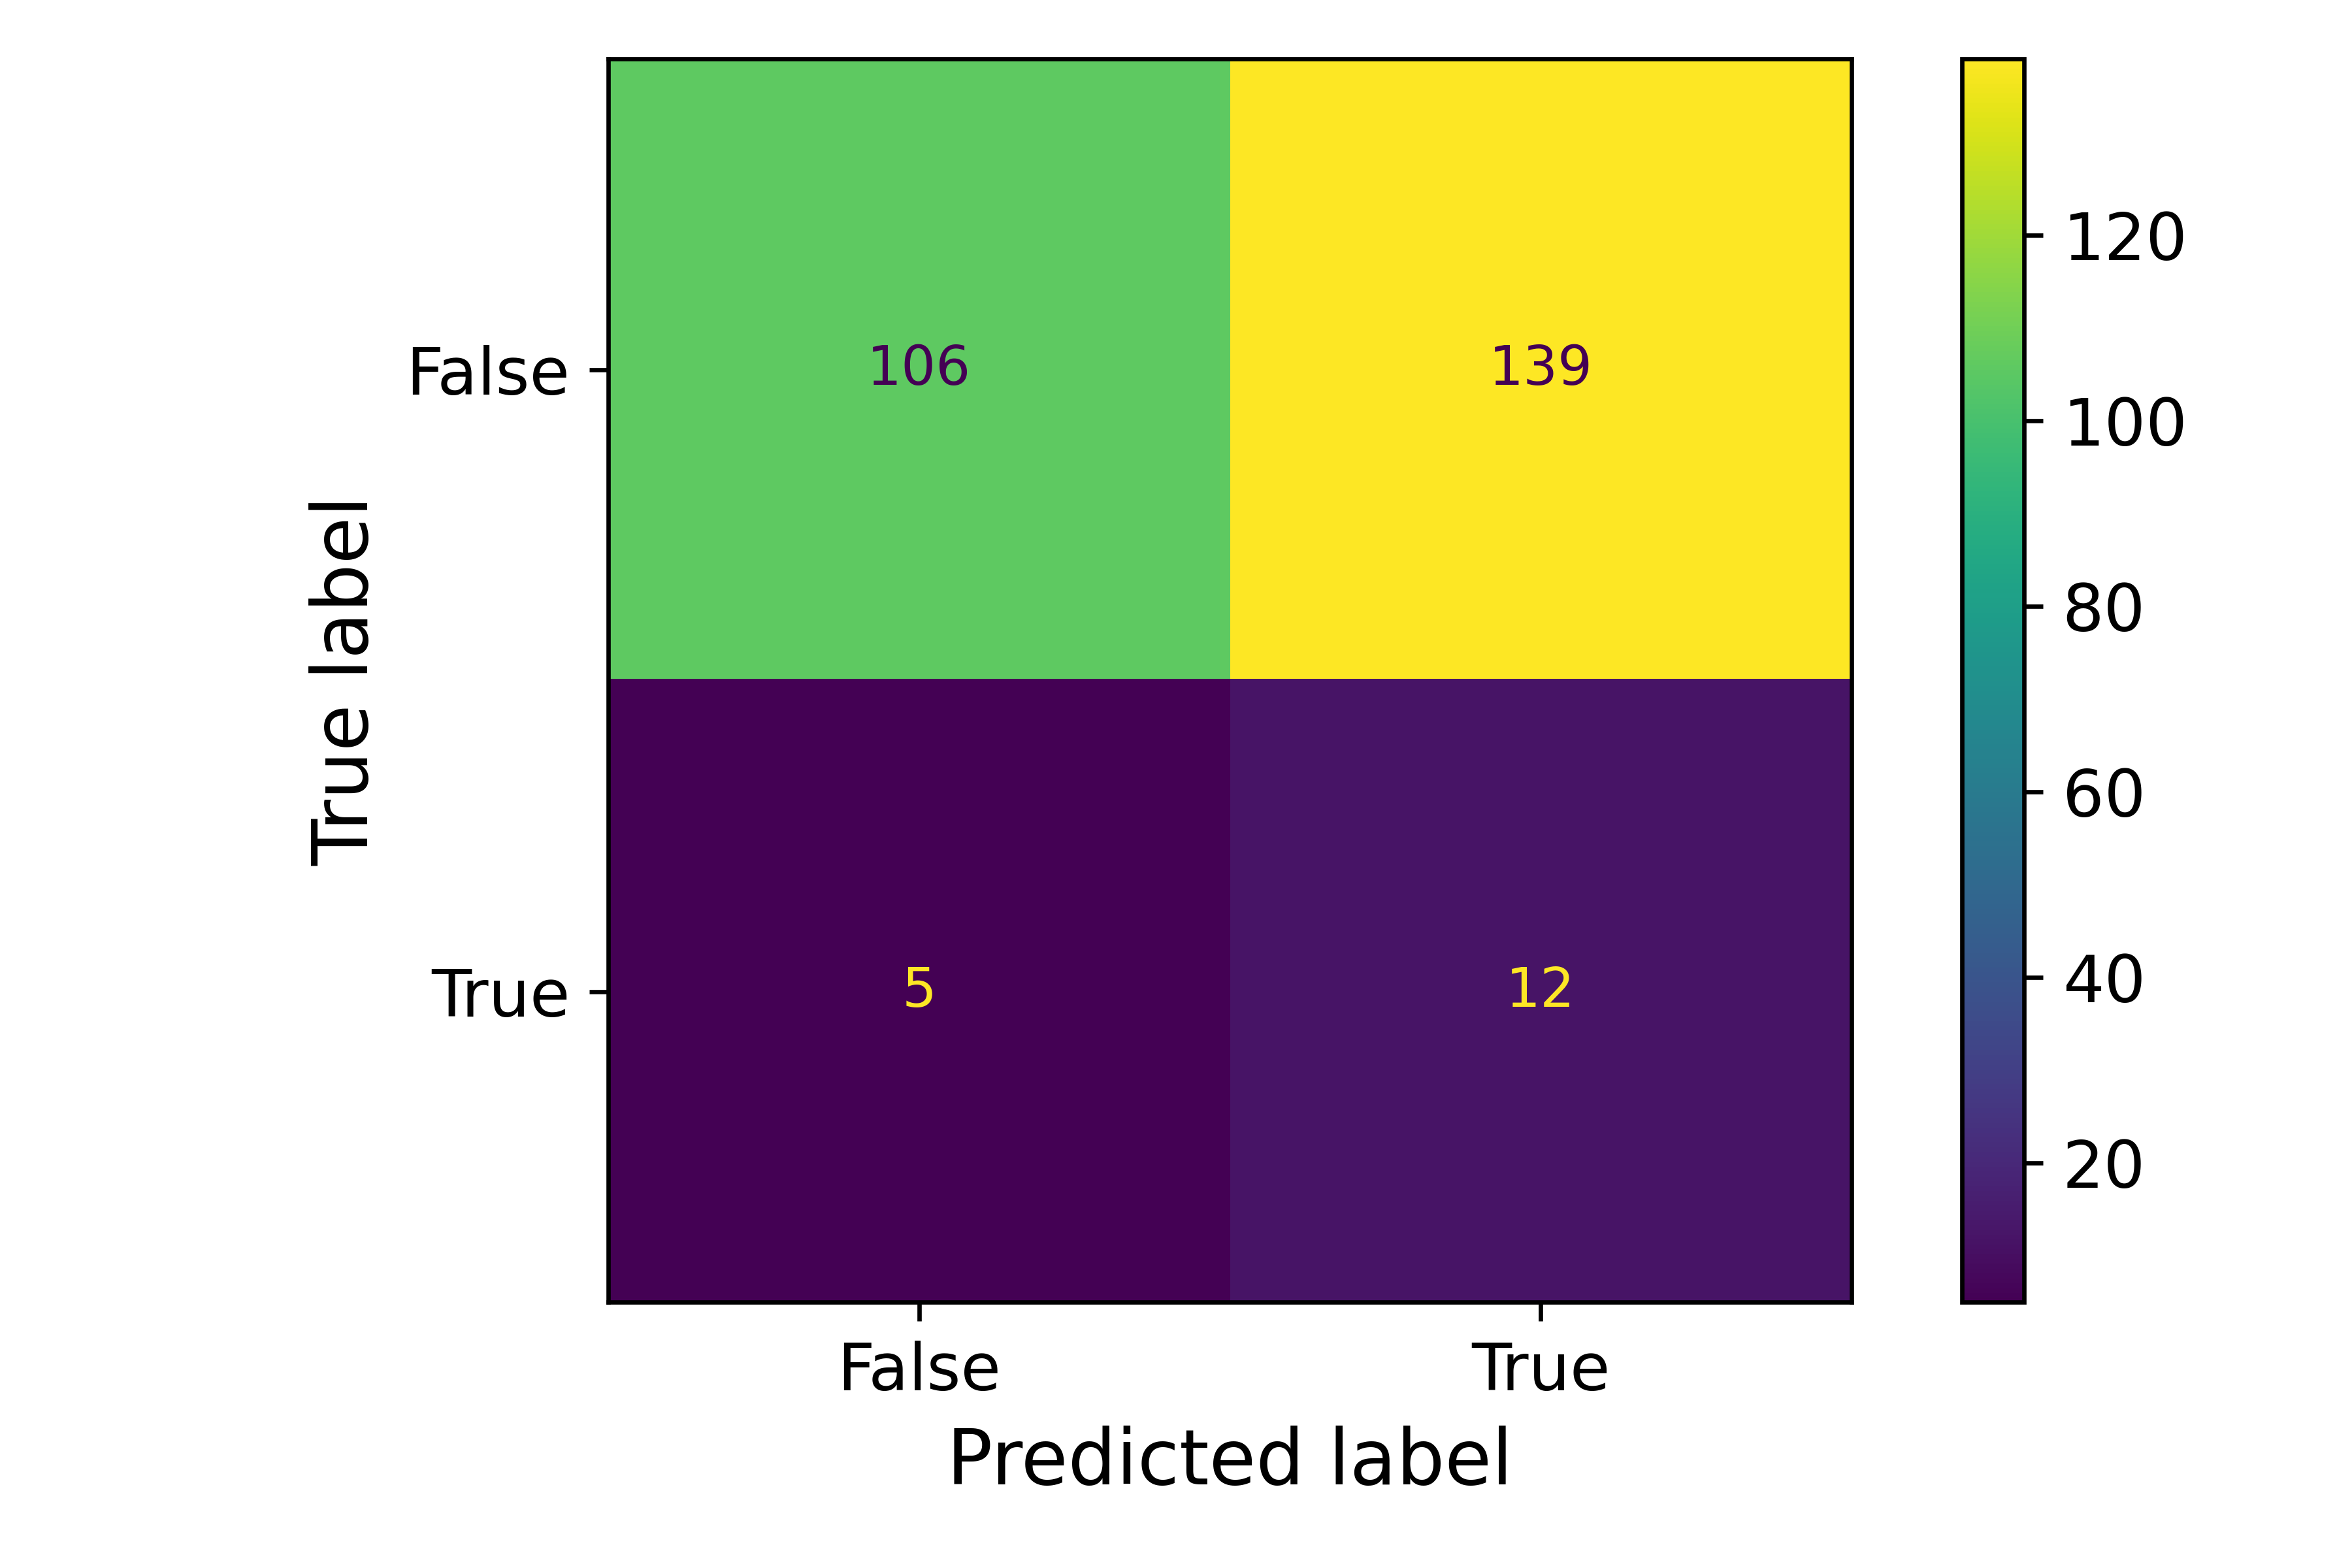
\includegraphics[scale=0.6]{../figure/NaiveBayesConfusionMatrix.png}
    \caption{Matrice di confusione Naive Bayes}
    \label{fig:CMNB}
\end{figure}
    
\begin{figure}[ht]
    \centering
    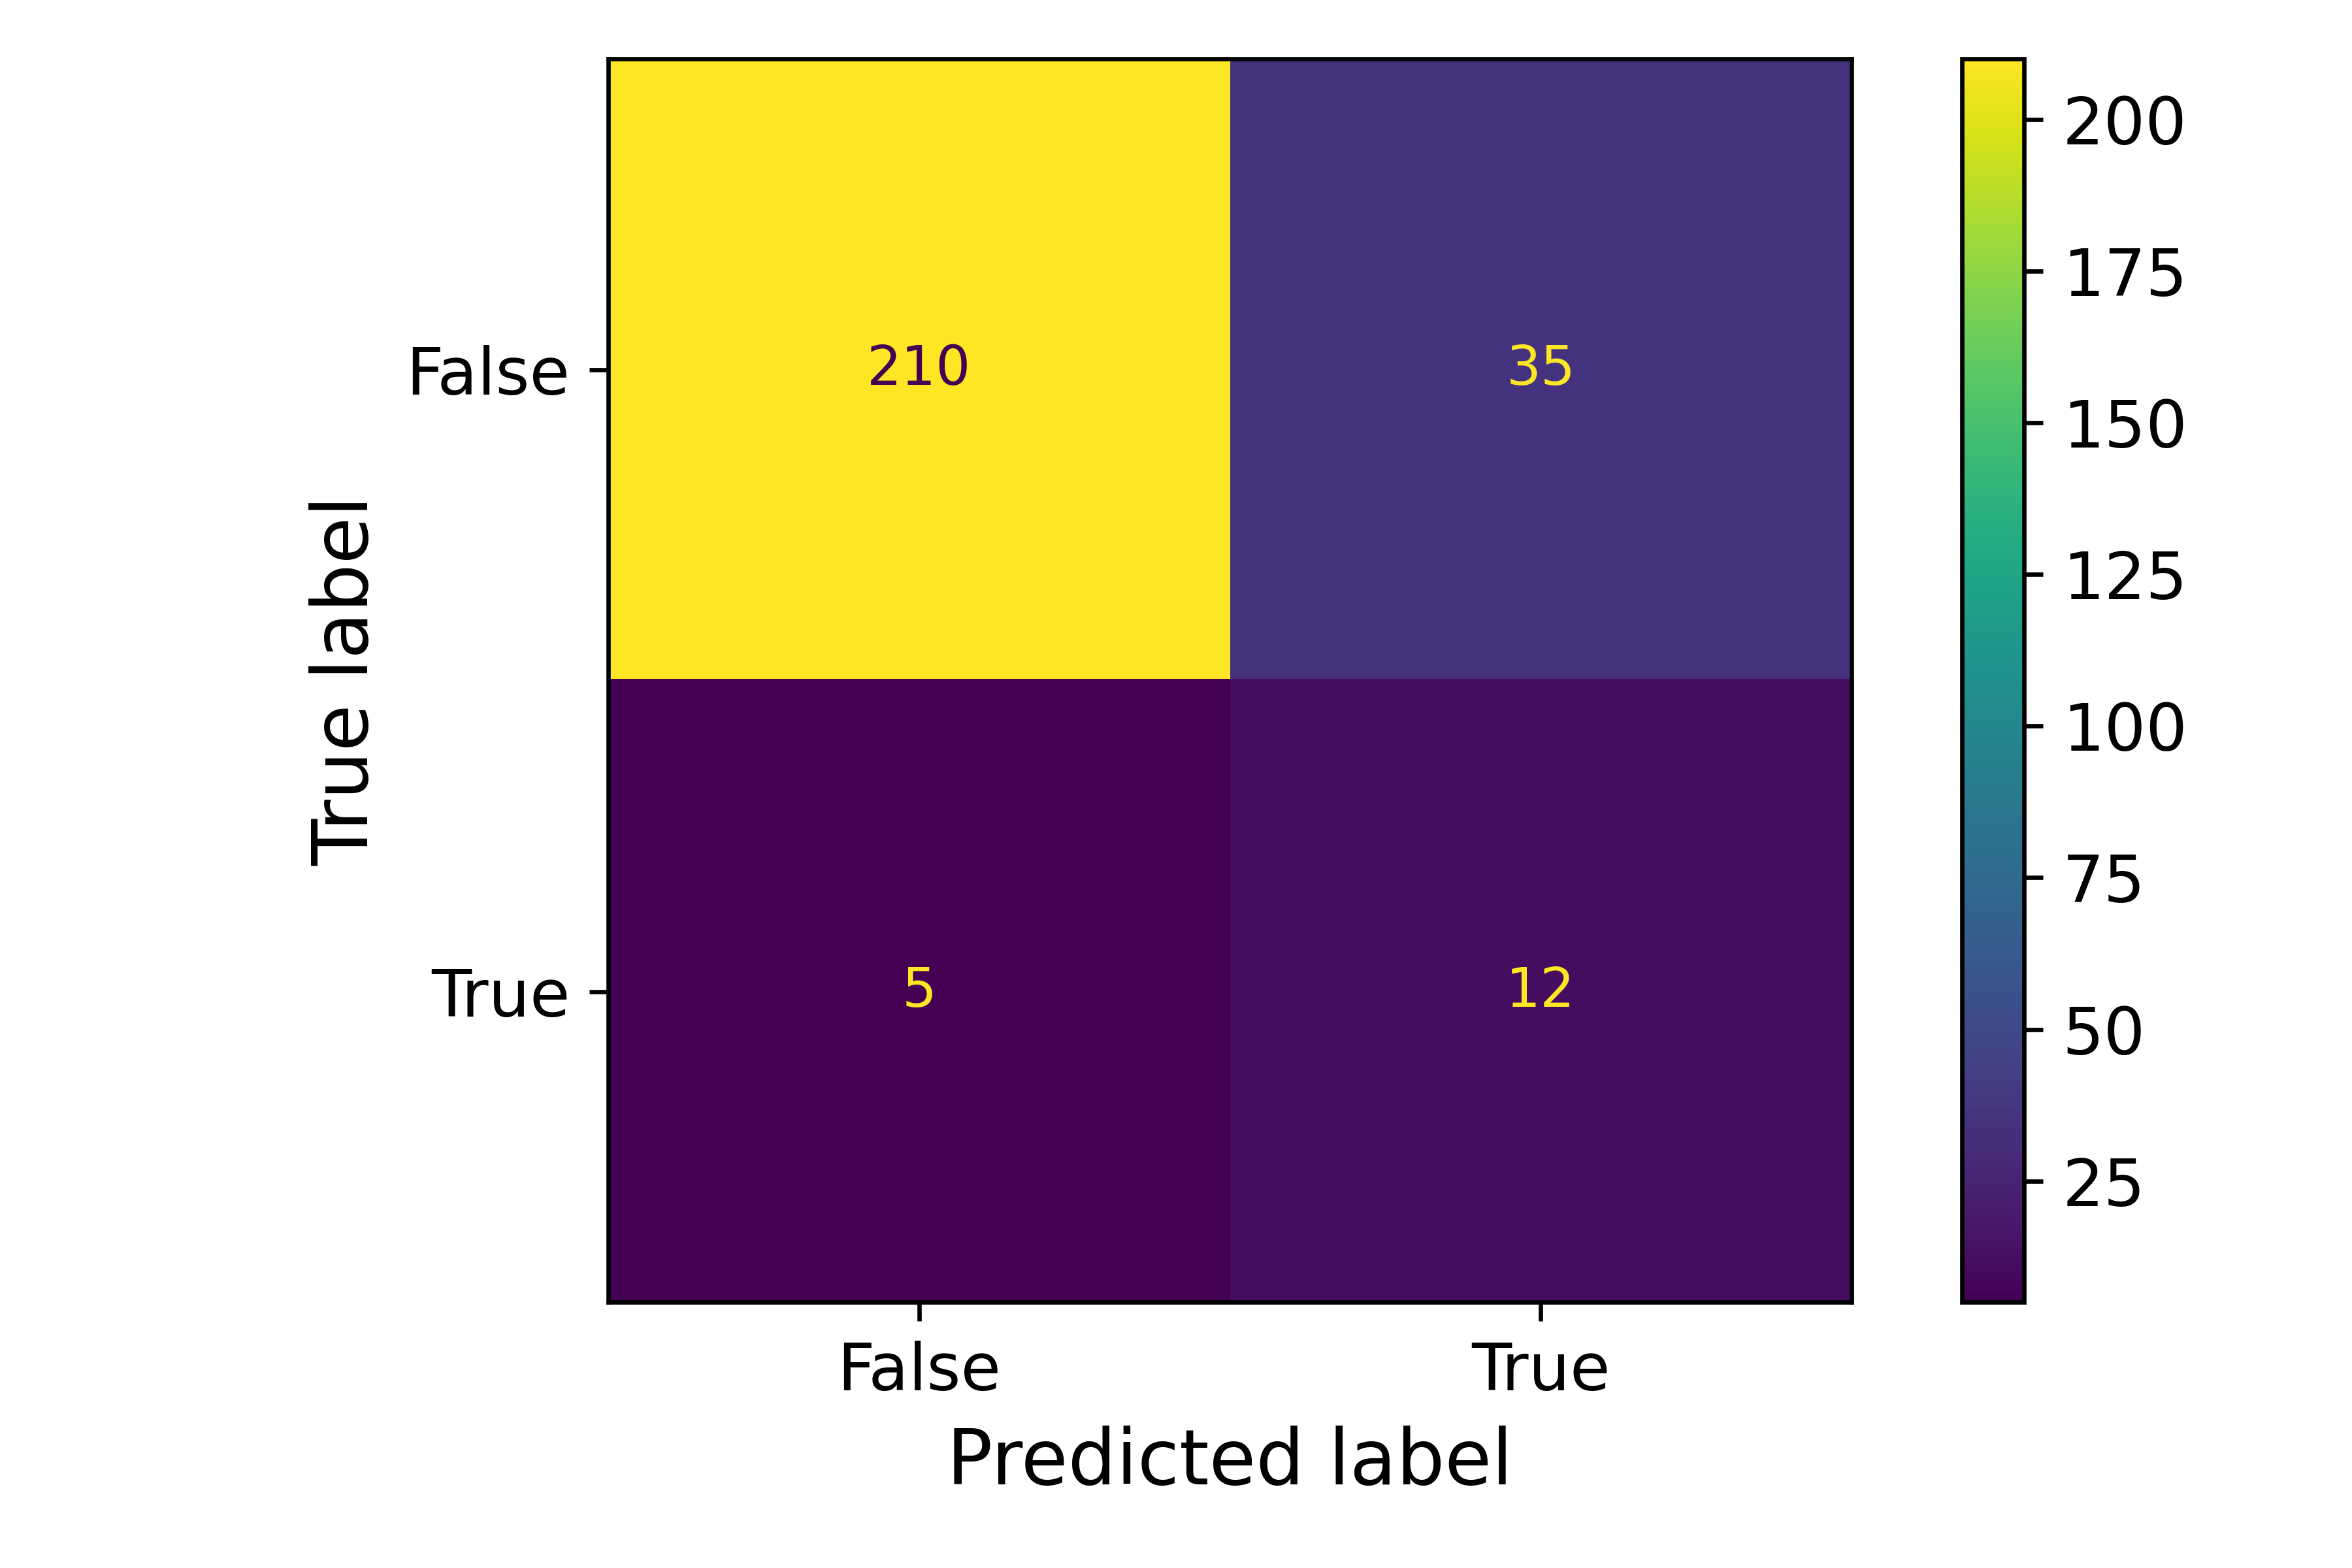
\includegraphics[scale=0.6]{../figure/DecisionTreeConfusionMatrix.png}
    \caption{Matrice di confusione Decision Tree}
    \label{fig:CMDT}
\end{figure}
Tra i dati più interessati emersi da questa analisi vediamo dalla matrice di confusione rappresentata dalla figura \ref{fig:CMNB} notiamo che il seguente classificatore in questo contesto ha una forte carenza per la predizione di file non vulnerabili, questo forte deficit influenza notevolmente il risultato di precision ciò spiega il motivo per cui questo modello ha riscontrato i livelli di precision più bassi di tutti i modelli implementati, questa forte carenza spiega anche il motivo per cui il seguente modello ha riscontrato il peggiore risultato di recall per la predizione di file non vulnerabili. Nonostante tutto notiamo che il classificatore Naive Bayes per i file vulnerabili ha predetto correttamente lo stesso numero di file dei classificatori che hanno raggiunto i risultati migliori e che sono Decision Tree \ref{fig:CMDT} e Random Forest \ref{fig:CMRF}. 
Il modello di predizione che invece ha registrato una bassissima capacità di predizione per file vulnerabili da come si evince dalla figura \ref{fig:CMSVMe} è stato il classificatore SVM con un numero di veri positivi migliore solo per una predizione nei confronti dei falsi positivi, nonostante ciò il classificatore ha ottenuto risultati migliori rispetto al classificatore Naive Bayes per la predizione dei file non vulnerabili, questo spiega il motivo per cui il SVM ha ottenuto risultati migliori in termini di precision.
Come detto in precedenza, analizzando i diversi classificatori notiamo che i risultati migliori ottenuti per la predizione di file vulnerabili sono analoghi per diversi classificatori, quindi il risultato migliore in termini di precision è legato al classificatore che ha una capacità predittiva maggiore per i file non vulnerabili, infatti come si nota dalla figura \ref{fig:CMRF} il classificatore Random forest ottiene i migliori risultati per la predizione di file non vulnerabili, ciò gli ha permesso di raggiungere i migliori risultati assoluti per il livello di precision.

\begin{figure}[]
    \centering
    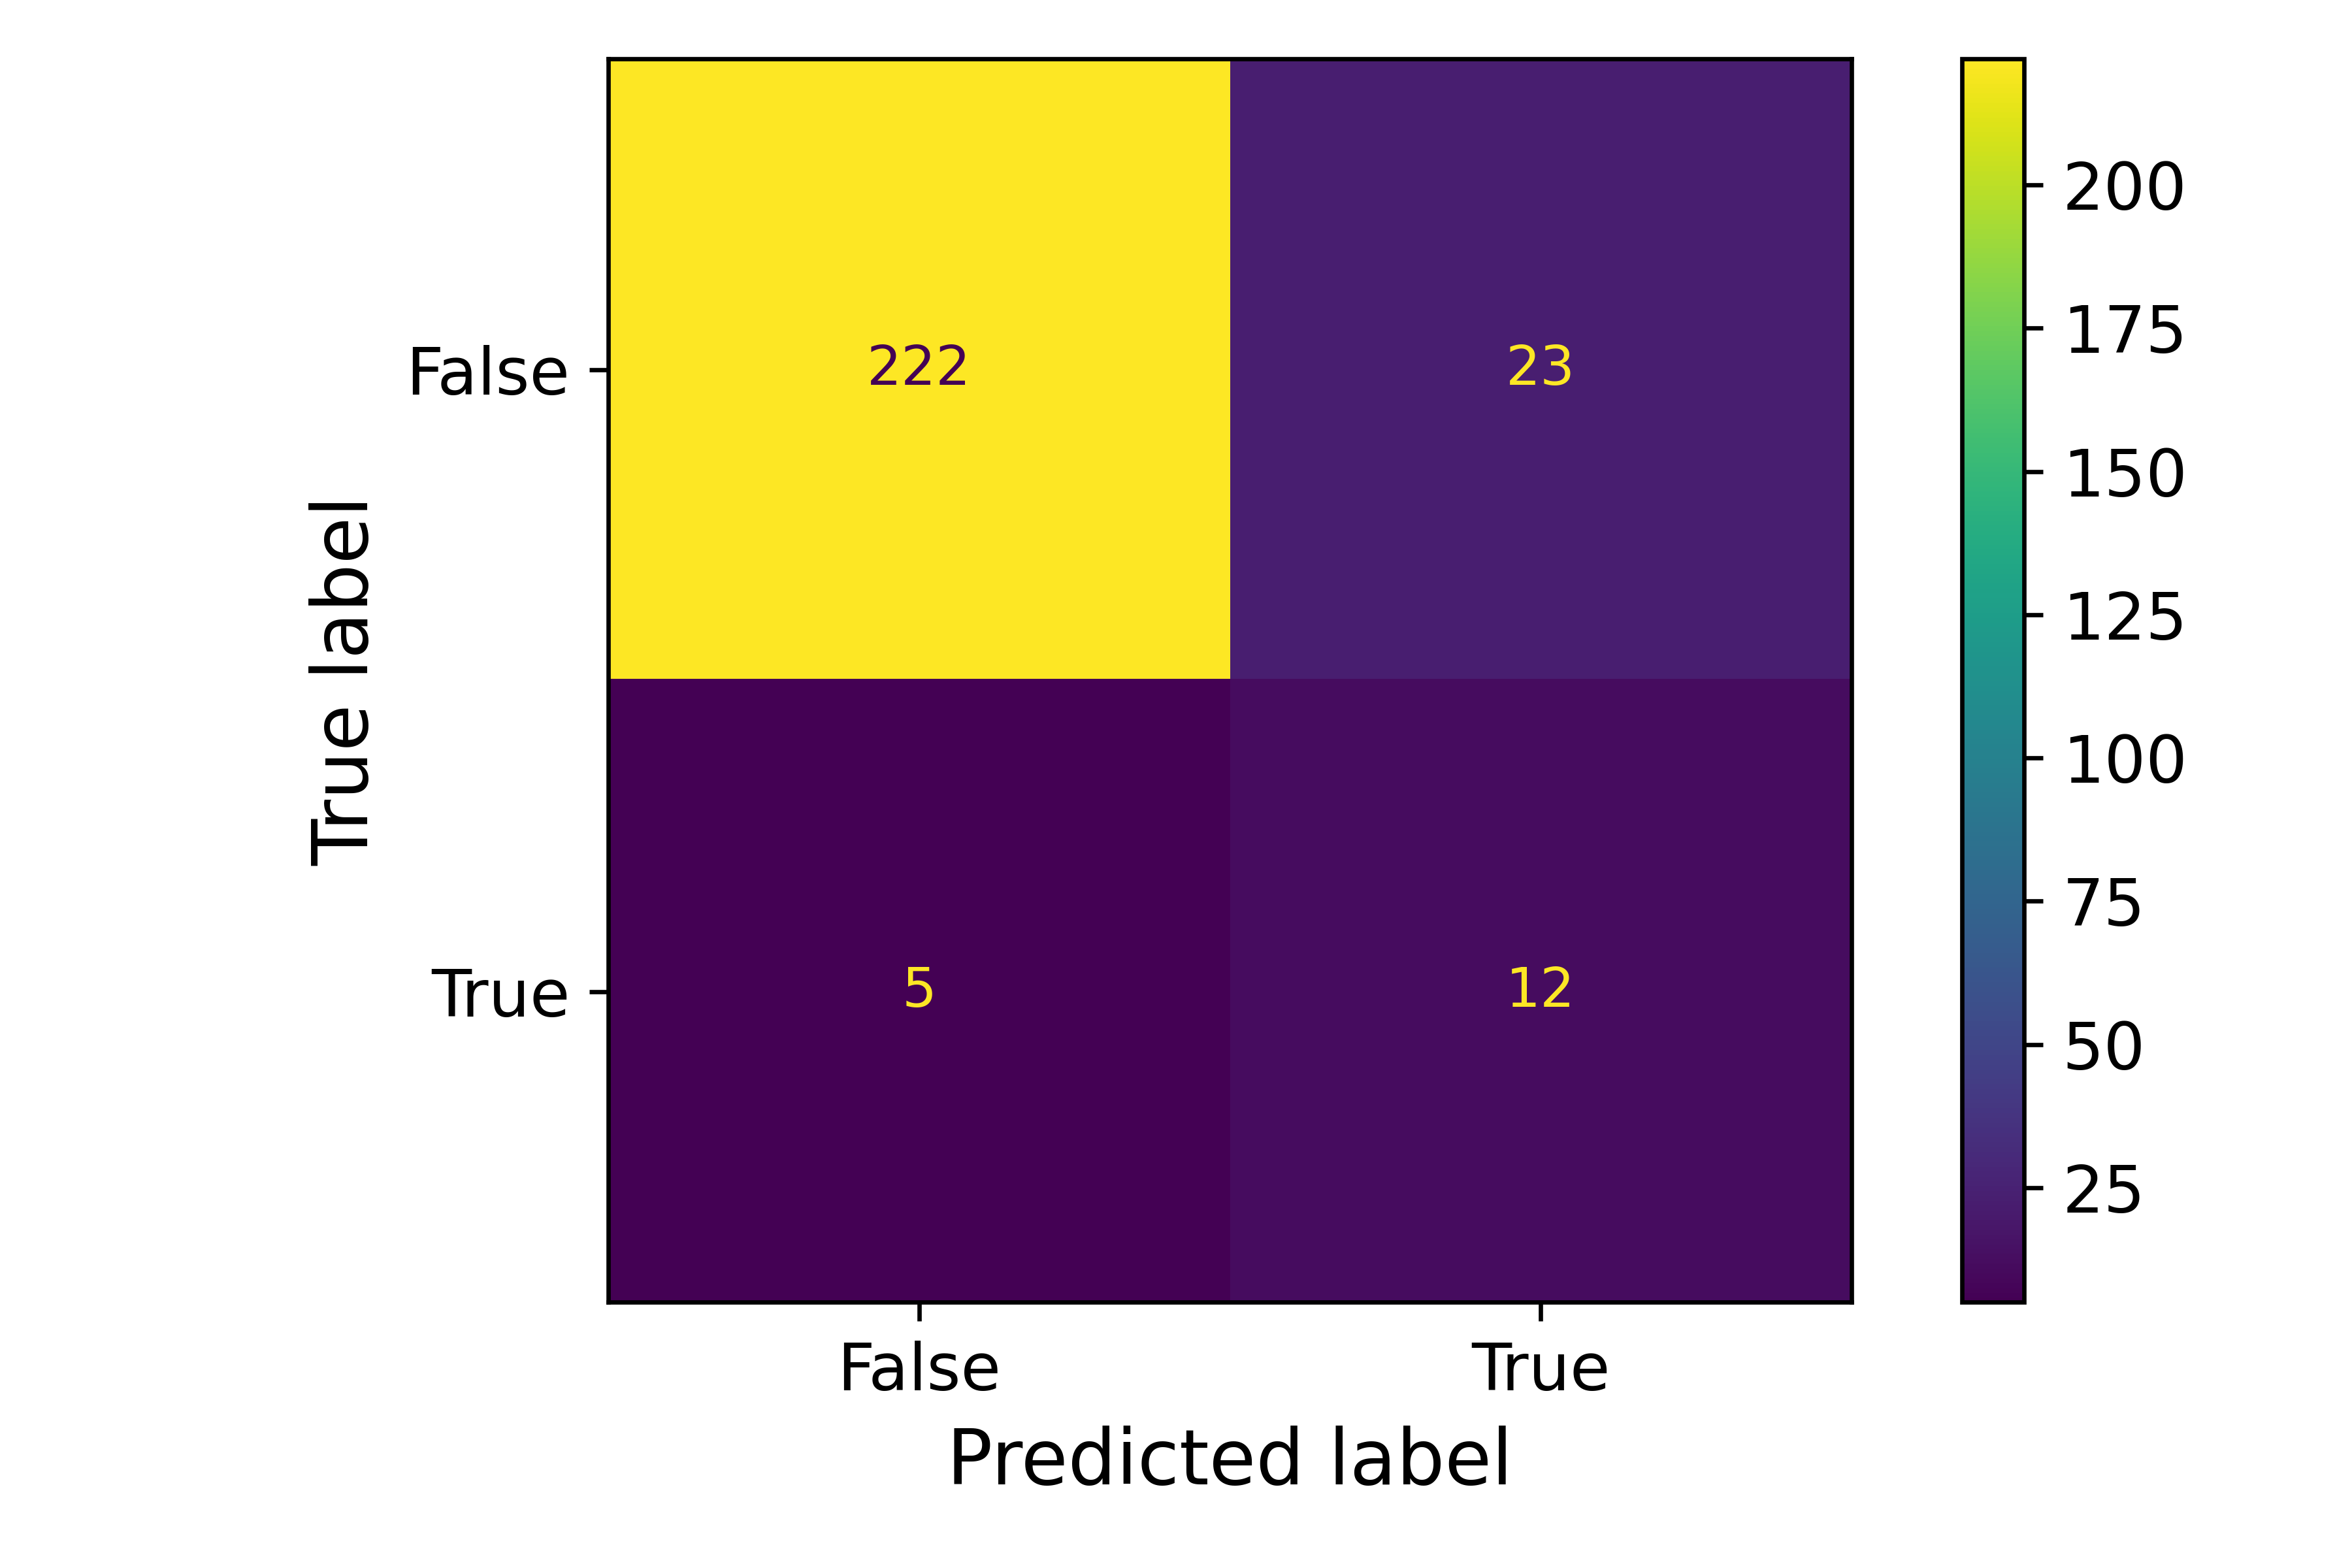
\includegraphics[scale=0.6]{../figure/RandomForestConfusionMatrix.png}
    \caption{Matrice di confusione Random forest}
    \label{fig:CMRF}
\end{figure}

\begin{figure}[!ht]
    \centering
    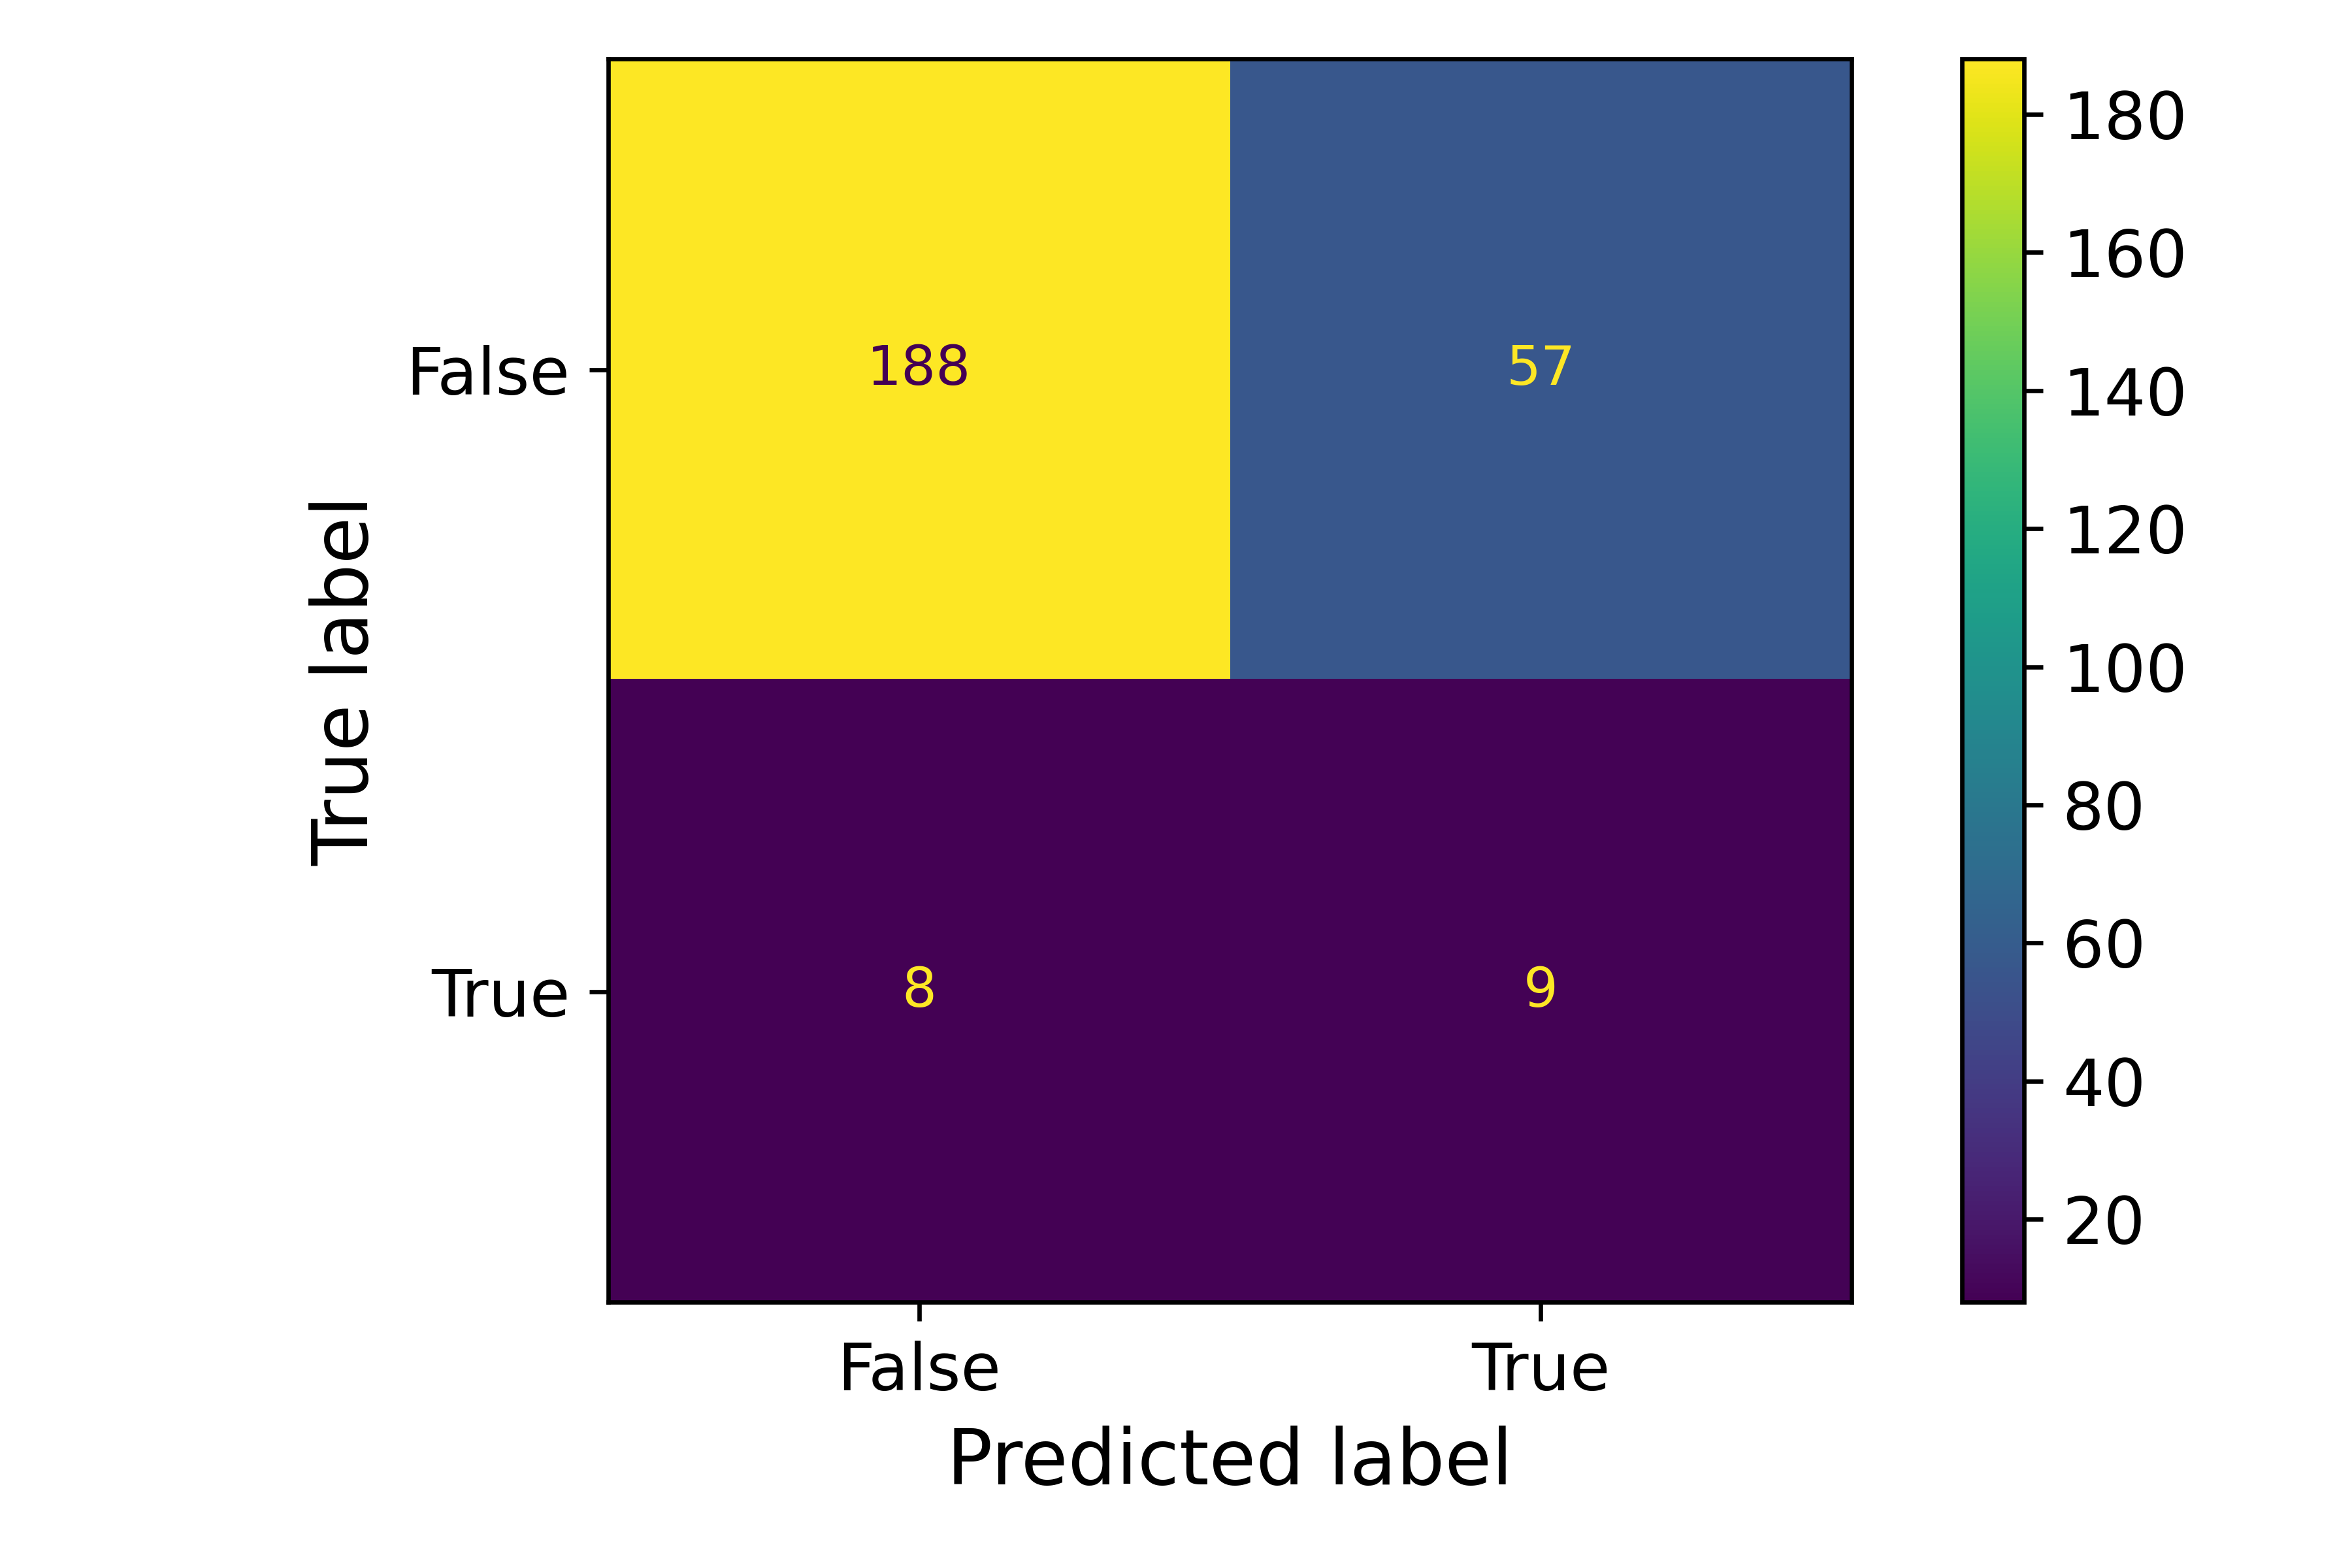
\includegraphics[scale=0.6]{../figure/SVMConfusionMatrix.png}
    \caption{Matrice di confusione SVM }
    \label{fig:CMSVMe}
\end{figure}

Dalle seguenti analisi possiamo osservare come i diversi classificatori operano ottenendo in alcuni casi risultati molto diversi tra loro. Nel ambito della predizione come si evince da questo studio e confermato da studi precedenti analizzati nel capitolo \ref{1cap:background} possiamo notare i classificatori più prestazionali per la predizione di vulnerabilità software sono quelli che prevedono la costruzione di uno o più alberi decisionali. Mentre il classificatore nel mio contesto che ha registrato performance più deludenti è stato il Naive Bayes, questo mostra come l'individuazione delle vulnerabilità software attraverso metriche software non è legato da fattori probabilistici. 

\begin{figure}[]
    \centering
    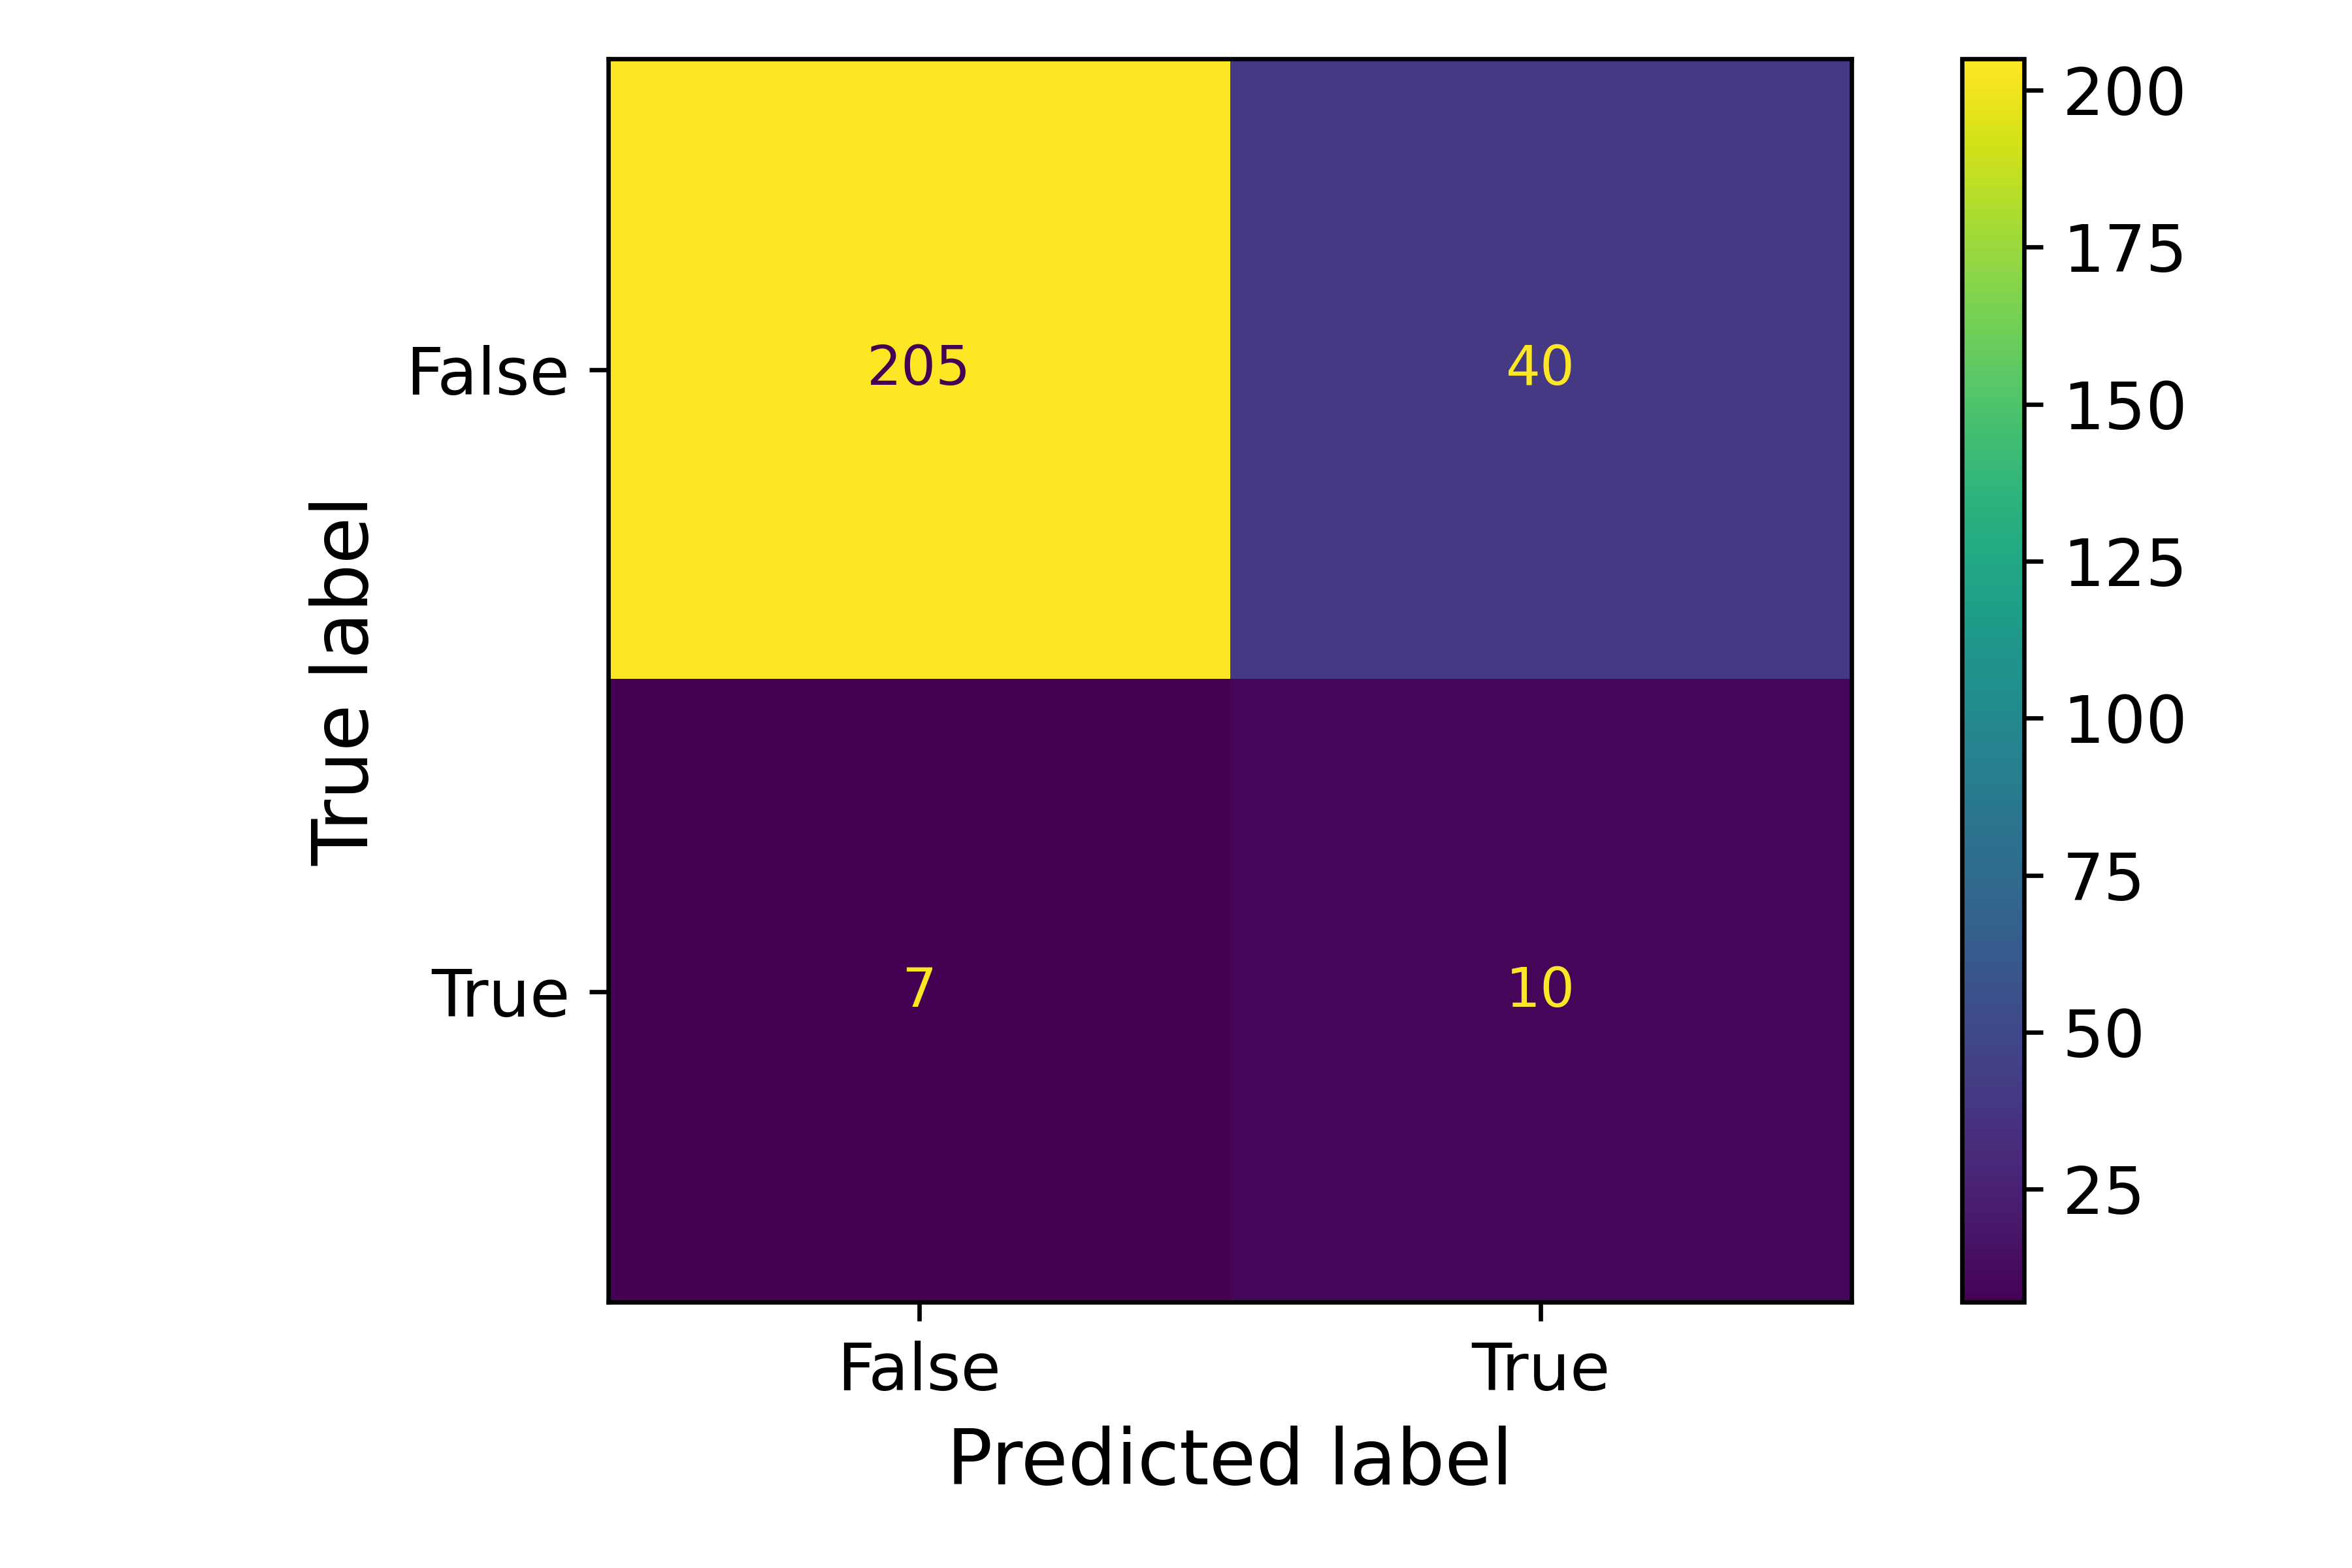
\includegraphics[scale=0.6]{../figure/AdaBoostConfusionMatrix.png}
    \caption{Matrice di confusione Ada Boost}
    \label{fig:CMAB}
\end{figure}


\newpage
